\chapter{学生实验}

\section{观察磁铁对电流的作用}

这个实验我们先用左手定则来判断磁场对电流的作用力
的方向,然后再用实验验证.

如图~\ref{fig_C_10-1} 所示,将矩形线圈悬挂在支架上,线圈的$AB$边
悬在蹄形磁铁的两极间.按照图~\ref{fig_C_10-1} 把电路连接好.
\begin{figure}[htbp]
    \centering
    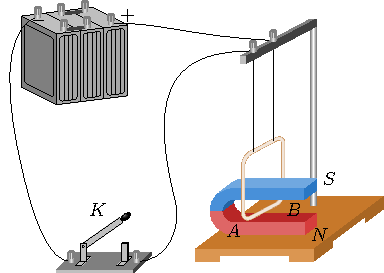
\includegraphics{fig/C/10-1.pdf}
    \caption{}\label{fig_C_10-1}
\end{figure}

根据电键闭合后$AB$边中的电流方向和$AB$边所在处的磁
场方向,用左手定则判断出磁场对$AB$边的作用力的方向.
合上电键$K$,观察$AB$边向哪个方向运动,与你判断的是否一致.
注意:只要看出了$AB$边的运动方向就要立即断开电键,
以免电池或线圈烧坏.
下面的实验也要这样.

把与电池正、负极连接的两条导线交换一下,改变$AB$边
中的电流方向,用左手定则判断出磁场对$AB$边的作用力的方向.
合上电键$K$,观察$AB$边向哪个方向运动,与你判断的
是否一致.$AB$边的受力方向与上一次比较改变没有?

把磁铁的$N$、$S$极调换一下,改变磁场的方向,先用左手
定则判断出磁场对$AB$边的作用力的方向,然后再做实验,看
一看与你判断的是否一致.
$AB$边的受力方向与上一次比较
改变了没有?

同学们自己设计一个表格,在每次实验前,先将$AB$边中
的电流方向以及磁铁的磁场方向填入表中,再根据实验时$AB$
边的运动方向,把磁铁对电流的作用力的方向填入表中.

\section{研究电磁感应现象}

关于感生电流产生的条件,我们已经随同老师一起做过
实验,现在用图~\ref{fig_C_2-3} 所示的装置来研究怎样判断感生电流的方向.
为了加强实验效果,这里用的螺线管$A$带有铁芯.

首先查明电流表指针的偏转方向和螺线管中电流方向的
关系,然后把蓄电池(或其他低压电源)、开关和螺线管$A$串联
成一个电路,把电流表和螺线管$B$串联成另一个电路.

接通电源,给螺线管$A$通电,然后把它插入螺线管$B$中,
停留一会儿再取出来.同时注意,当螺线管$A$在插入或取出
时,跟螺线管$B$相连的电流表的偏转方向,并记下$B$中感生电
流的方向.

改变螺线管$A$中的电流方向,重做上面的实验,观察跟螺线
管$B$相连的电流表的偏转方向,并记下$B$中感生电流的方向.

把螺线管$A$放在螺线管$B$中不动,观察在给螺线管$A$通
电和断电的瞬间,跟螺线管$B$相连的电流表的偏转方向,并记
下$B$中感生电流的方向.
改变螺线管$A$的通电方向,再观察在
通电和断电的瞬间,跟螺线管$B$相连的电流表的偏转方向,并
记下$B$中感生电流的方向.

分析你的实验并回答下列问题:
\begin{enumerate}
    \item 螺线管$B$内部的磁场增强时,$B$中感生电流的磁场
方向怎样?螺线管$B$内部的磁场减弱时,$B$中感生电流的磁
场方向怎样?
\item 归纳出判断感生电流方向的规律.
\end{enumerate}

\section{用示波器观察交流电的波形}
这个实验是用示波器来观察交流电的波形.
我们讲过,
示波器自己能发出正弦交流信号.
我们就先观察示波器自己
的正弦交流信号.
然后再观察从信号源输入的交流信号.

开机前,先把辉度调节旋钮反时针转到底,衰减旋钮置于
正弦符号“\tikz \draw[x=.7ex,y=1ex] (0,0) sin (1,1) cos (2,0) sin (3,-1) cos (4,0)--(0,0);”档,Y增益旋钮顺时针转到底,扫描范围置于$10 \sim 100$赫兹档,其余各个旋钮置于中间位置.打开电源开关,
经预热后,顺时针旋转辉度调节旋钮,可以看到不稳定的不一
定清晰的波形.
调整聚焦调节和辅助聚焦旋钮,使图线清晰.
调整垂直位移和水平位移旋钮,使图象位置适中.
调整X增
益旋钮,使图象大小合适.作好这些准备工作后,把同步开关
置于“$+$”位置,把扫描微调旋钮先顺时针转到底再慢慢地反
时针旋转,当转到某一位置时,可以看到一个稳定的完整的正
弦波形(图~\ref{fig_C_10-2a}).
屏上还同时出现的水平亮线是扫描的回扫线.
把同步开关置于“$-$”位置,又可看到波形改变半个周期
(图~\ref{fig_C_10-2b}).如果扫描频率恰好是信号频率的$1/n$($n$为整
数),将可看到稳定的$n$个完整波形,继续慢慢地反时针旋转
扫描微调旋钮,减小扫描频率,就可以看到屏上出现稳定的两
个、三个正弦波形.

\begin{figure}[htbp]
    \centering
    \begin{subfigure}{0.4\linewidth}
        \centering
        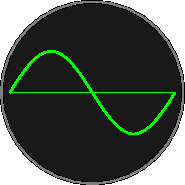
\includegraphics{fig/C/10-2a.pdf}
        \caption{}\label{fig_C_10-2a}
    \end{subfigure}
    \hfil
    \begin{subfigure}{0.4\linewidth}
        \centering
        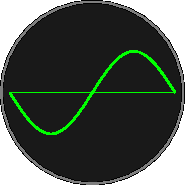
\includegraphics{fig/C/10-2b.pdf}
        \caption{}\label{fig_C_10-2b}
    \end{subfigure}
    \caption{}\label{fig_C_10-2}
\end{figure}



现在再来观察从信号源输入的交流信号.我们用的信号
源是J2465型学生信号源.
这种信号源可以输出低频、高频正
弦交流信号和高频调幅信号(在第\ref{chapter-electromagnetic-oscillations-and-waves}章将讲到什么是调幅信
号).J2465型学生信号源的面板如图~\ref{fig_C_10-3} 所示,下面先介
绍它的使用方法.

\begin{figure}[htbp]
	\centering
	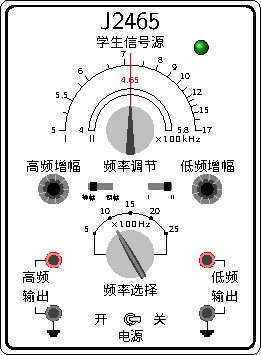
\includegraphics{fig/C/10-3.pdf}
	\caption{J2465型学生信号源的面板}\label{fig_C_10-3}
\end{figure}



低频正弦交流信号从右边的两个低频输出接线柱输出.
它们的上边是低频增幅旋钮,顺时针旋转它,低频输出的电压
连续增大.中间的频率选择旋钮用来改变低频输出的频率;
它有五档:500,1000,1500,2000和2500赫.

高频信号从左边的两个高频输出接线柱输出.它们的上
边是高频增幅旋钮,顺时针旋转它,高频输出的电压连续增
大.上边的频率调节旋钮用来连续改变高频输出的频率.
当右边的选择开关在位置“I”时,频率改变范围是$500 \sim 1700$千
赫;在位置“II”时,是$400 \sim 580$千赫.

需要高频正弦交流信号时,左边的选择开关应置于“等
幅”位置.当这个选择开关置于“调幅”位置时,从高频输出接
线柱输出的是高频调幅信号.调幅度的大小用低频增幅旋钮
来调节.
调制信号的频率用频率选择旋钮来选择.

让我们观察从信号源输入的低频正弦信号.
为此,先用
导线把信号源的两个低频输出接线柱跟示波器的“Y输入”和
“地”两个接线柱连接上;把信号源的低频增幅旋钮转到中间
位置;把示波器的衰减旋钮从正弦符号档转到最高档.
打开它
们的电源开关,示波器的准备工作跟前面相同.
逐步减小衰减
档并调整Y增益,使图象的竖直幅度适宜.然后根据输入的
信号频率选择适当的扫描范围并调整扫描微调,就可以看到
稳定的整数个完整的波形.
再慢慢调整扫描微调,可以看到
波形数发生改变.
调整X增益,可以看到波形的水平幅度的
改变.把同步开关从“$+$”位置扳到“$-$”位置,可以看到波形
改变半个周期.旋转信号源的低频增幅旋钮,观察波形的竖
直幅度的改变.在观察过程中,必要时应随时调整辉度调节、
聚焦调节和辅助聚焦,使图象亮度适宜,图线清晰.

利用示波器还可以测出输入的交流信号的电压的最大值
并进而算出它的有效值.测量时应注意把Y增益旋钮顺时针
旋转到底,还应根据衰减乘以相应的倍数.你在实验中,当低
频增幅旋钮转到最大时,信号电压的最大值和有效值各是多
少?

改变输入信号的频率,再次进行各项调整和观察.

如果有多余的时间,还可以继续观察高频正弦信号和高
频调幅信号.
各项调整方法跟观察低频正弦信号时基本相同.

\section{用示波器观察交流电的整流和滤波}\label{sec_C_app_01-4}

这个实验通过示波器观察波形来了解整流滤波电路的作
用.

图~\ref{fig_C_10-4} 是一个带$\pi$型滤波器的半波整流路.交流电源
的电压,滤波电容器$C_1$、$C_2$的电容,电阻$R$的阻值,都是根据
负载$R_{\text{负}}$的要求选定的.$C_1$、$C_2$越大,滤波效果越好.$R$大些,
滤波效果好些,但电压损失也大些.
图中的数据可作参考.
这个电路可提供$5 \sim 6$伏特的直流电.
\begin{figure}[htbp]
    \centering
    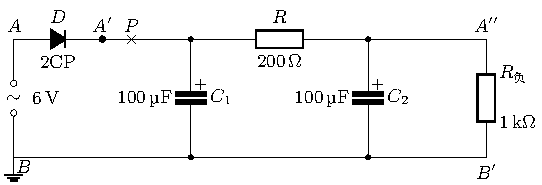
\includegraphics{fig/C/10-4.pdf}
    \caption{}\label{fig_C_10-4}
\end{figure}

在一张适当大小的白纸上,画出图中所示的电路,并标出
各个元件的规格.把这张电路图平铺在一块铁板上,选取你
需要的实验元件(图~\ref{fig_C_10-5} 所示的是专为实验用的几种元件).
将各个元件放在电路图标出的位置上(应注意二极管和电解
电容器的正负极不要接错).
用导线将各元件按照电路图连
接起来.
为了观察整流前后的波形,$P$点先不要接通.

\begin{figure}[htbp]
    \centering
    \begin{subfigure}{0.3\linewidth}
        \centering
        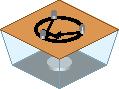
\includegraphics{fig/C/10-5a.pdf}
        \caption{晶体三极管}\label{fig_C_10-5a}
    \end{subfigure}
    \hfil
    \begin{subfigure}{0.2\linewidth}
        \centering
        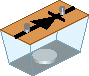
\includegraphics{fig/C/10-5b.pdf}
        \caption{晶体二极管}\label{fig_C_10-5b}
    \end{subfigure}
    \hfil
    \begin{subfigure}{0.2\linewidth}
        \centering
        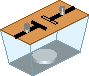
\includegraphics{fig/C/10-5c.pdf}
        \caption{电容}\label{fig_C_10-5c}
    \end{subfigure}
    \hfil
    \begin{subfigure}{0.2\linewidth}
        \centering
        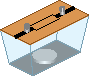
\includegraphics{fig/C/10-5d.pdf}
        \caption{电阻}\label{fig_C_10-5d}
    \end{subfigure}
    \caption{实验用的元件.元件装在透明塑料盒内,盖上画着元件的符号,并有弹簧式的接
    线头,盒底有块磁铁,使元件能平稳地安放在实验用的铁板上.}\label{fig_C_10-5}
\end{figure}

电路检查无误后,即可接上6伏的交流电源,用示波器观
察波形.先把负载$R_{\text{负}}$改接在$A$点和“地”(即$BB'$导线)之间,
把$A$点接示波器的Y输入,$BB'$导线接示波器的“地”,观察整
流前的交流电压波形.
再把负载$R_{\text{负}}$改接在$A^{\prime}$点和“地”之
间,把$A'$点接示波器的Y输入,$BB'$导线仍然接示波器的
“地”,观察整流后的电压波形.
然后接通$P$点,把负载$R_{\text{负}}$接
在图~\ref{fig_C_10-4} 所示的位置,把$A^{\prime\prime}$点接示波器的Y输入,$BB'$导线
仍然接示波器的“地”,观察滤波后的电压波形.
在观察波形
时,在坐标纸上把三种波形记录下来,以便比较.

有兴趣的同学还可以改变电容器$C_1$、$C_2$和电阻$R$的数
值,观察$A''$点对“地”的电压波形的变化,研究它们对滤波效
果的影响.

\section{研究变压器的作用}
这个实验利用变压器模型来研究变压器的作用.

这个变压器模型有三个线圈,线圈I为120匝,线圈II为
240匝,线圈III为60匝.
现在拿线圈I作原线圈,线圈III作
副线圈,把它们套在一起,将硅钢片插入原、副线圈中,这样就
装成了一个降压变压器.

记下原线圈的匝数$n_1$和副线圈的匝数$n_2$.将原线圈的
两端接低压交流电源,副线圈的两端跟小电灯泡相连.
用交流电压表分别测量原、副线圈两端的电压$U_1$和$U_2$,记下测得
的数据.
看看它们的电压比
$U_1/U_2$跟匝数比$n_1/n_2$
有什么关系.

用交流电流表分别测出原、副线圈中的电流$I_1$和$I_2$,记
下测得的数据.
看看原、副线圈中的电流比$I_1/I_2$
跟它们的匝数比$n_1/n_2$有什么关系.

根据测得的原、副线圈的电压和电流的数值,算出变压器
的输入功率$U_1I_1$和输出功率$U_2I_2$.
你这个变压器的效率是
多少?

在输出电路中再并联几个小灯泡.负载增加后,副线圈
中的电流增大了,原线圈中的电流怎样变化?输出功率和输
入功率怎样变化?

拆开变压器,换上线圈II作副线圈,然后再将硅钢片插
入,装成一个升压变压器.
按上面的步骤重做一遍实验.

根据你的实验,回答下面的问题:
\begin{enumerate}
    \item 变压器原、副线圈两端的电压跟它们的匝数有什么关系?
    \item 变压器原、副线圈中的电流跟它们的匝数有什么关系?
    \item 变压器的输出电流改变时,输入电将怎样改变?输
出功率改变时,输入功率将怎样改变?输出功率和输入功率
是否相等?为什么?
\end{enumerate}

\section{安装简单的收音机}
我们用方框图已经讲过简单晶体管收音机的工作原理.
现在来连接这种收音机的电路,学习它的安装和调试方法.

图~\ref{fig_C_10-6} 是一个两管收音机的线路图,它包括调谐、高频
放大、检波、低频放大四个部分,图中已经用虚线隔开.
图中
的$R_1^*$和$R_2^*$叫做偏流电阻.
\begin{figure}[htbp]
    \centering
    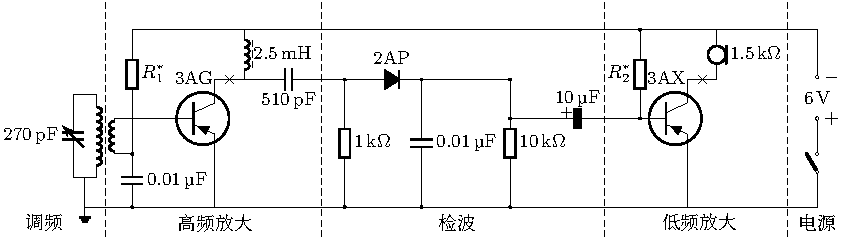
\includegraphics{fig/C/10-6.pdf}
    \caption{简单收音机的线路图}\label{fig_C_10-6}
\end{figure}

按照图~\ref{fig_C_10-6} 连接电路,连接的方法跟实验\ref{sec_C_app_01-4}相同.先在
白纸上画出电路图,然后根据规格选取需要的元件,放在纸上
摆好,再用导线把它们连接起来.偏流电阻$R_1^*$和$R_2^*$的阻值
待定,可以先空着,等调试后再连入.

连接完毕,要按照电路图全面仔细检查一遍,确认无误
后,即可接上电源进行调试.

对本机的调试,就是调整两个三极管的偏流电阻.
把毫安表或万用电表的毫安档接入三极管的集电极电路(图中画
“$\times$”号处),用20千欧的固定电阻和470千欧的电位器串联
起来暂代偏流电阻连入电路.
调节电位器,使高频三极管集电
极电流为1毫安左右,低频三极管集电极电流为2毫安左右.
然后取下串联的固定电阻和电位器,用万用电表分别测出它
们的总电阻,用阻值相同的固定电阻连入电路,调试工作就完
成了.

调试好以后,即可调节可变电容器来试听电台的广播.
本机的灵敏度不高,在广播电台较远时可能收听不到.遇到这
种情况,可以用信号源发出高频调幅信号来代替广播电台,这
时从耳机里可以听到嗡嗡的调制信号的音频交流声.

\section{测定玻璃的折射率}

在这个实验里,我们用两面平行的玻璃砖来测定玻璃的
折射率.
从第\ref{chapter-reflection-and-refraction-of-light}章\ref{sec_C_5-6}小节的例题可知,当光线斜射入两面平行的玻璃板
时,从玻璃板射出的光线传播方向不变,出射光线跟入射光线
相比,只有一定的侧移.只要我们找出跟某一入射光线对应的
出射光线,就能求出在玻璃中对应的折射光线,从而求出折射角.
再根据折射定律,就可以求出玻璃的折射率.
\begin{figure}[htbp]
    \centering
    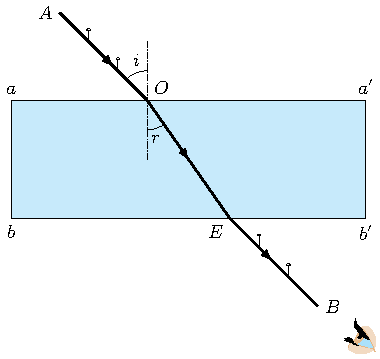
\includegraphics{fig/C/10-7.pdf}
    \caption{}\label{fig_C_10-7}
\end{figure}

实验的具体做法如下:照图~\ref{fig_C_10-7} 那样,先在一张白纸上
画直线$aa'$作为玻璃砖的一个界面,过$aa'$上的一点$O$画界面
的法线$NN'$,再画直线$AO$作为入射光线.
把长方形玻璃砖
放在白纸上,使它的长边跟$aa'$对齐,画出玻璃砖的另外一边
$bb'$.在直线$AO$上竖直插上两枚大头针$P_1$、$P_2$,透过玻璃砖观
察大头针$P_1$、$P_2$的像.
移动视线的方向,直到$P_1$的像被$P_2$的
像挡住.再在观察的这一侧插两枚大头针$P_3$、$P_4$,使$P_3$挡住
$P_1$、$P_2$的像,$P_4$挡住$P_3$和$P_1$、$P_2$的像.


记下$P_3$、$P_4$的位置.移去玻璃砖和大头针.
过$P_3$、$P_4$引直
线$EB$,与$bb'$交于$E$,$EB$就表示沿$AO$方向入射的光线通过
玻璃砖后传播的方向.连接$OE$,$OE$就是玻璃砖内折射光线
的方向.
入射角$i=\angle AON$,折射角$r=\angle EON'$.

用量角器量出入射角和折射角,从三角函数表中查出它
们的正弦值,把这些数据记在自己设计的表格里.

用上面的方法分别求出入射角是30$^\circ$、45$^\circ$、60$^\circ$时的折射
角,查出它们的正弦值,把得到的数据记在表格里.

算出不同入射角时
$\sin i/\sin r$
的比值,比较一下,看它们是否接
近于一个常数.求出几次测得的
$\sin i/\sin r$
的平均值,作为测得的
玻璃的折射率$n$.

\section{测定凸透镜的焦距}
测定凸透镜的焦距有各种不同的方法.
在这个实验里我
们用三种比较简单的方法来测定.

\subsection{平行光聚焦法}

平行于凸透镜主轴的光线,经凸透
镜折射后将会聚于焦点,利用凸透镜的这一特性,可以测出它
的焦距.方法是把凸透镜对着远处的光源(例如太阳),在透
镜的另一侧放一个光屏(或一张白纸),调节透镜和白纸间的
距离,直到屏上出现的光斑最亮最小为止.
这个光斑就是透
镜的焦点.
用直尺量出这时透镜到光斑间的距离,就得到凸
透镜的焦距.

\subsection{利用透镜成像公式}

把点燃的蜡烛、凸透镜、光屏照
图~\ref{fig_C_5-38} 那样放在光具座上,调整它们的高度,使烛焰和光屏的
中心位于凸透镜的主轴上(共轴).调节蜡烛和光屏到透镜的
距离,使光屏上呈现出烛焰的清晰的像,量出这时的物距和像
距,填入自己设计的表格中.

改变蜡烛到凸透镜的距离,按照上段的要求再做两次.
把测得的数据也填入表格中.

根据测得的三组数据,利用凸透镜的成像公式
\[\frac{1}{u}+\frac{1}{v}=\frac{1}{f} \]
算出三次得到的$f$值,求出它们的平均值,作为测得的凸透
镜的焦距.

\subsection{利用公式$f=(L^2-d^2)/4L$}\label{subsec_C_app_01-8-3}

从第\ref{chapter-reflection-and-refraction-of-light}章\ref{sec_C_5-12}小节的例题知道,如果保
持物体和光屏之间的距离$L$不变,在物体和光屏之间移动凸透
镜,使物体在光屏上先后两次成像,测出凸透镜的两个位置间
的距离$d$,那么凸透镜的焦距
\[f=\dfrac{L^2-d^2}{4L} \]
需要注意的是,用这
种方法测焦距时,一定要使$L>4f$,才能在光屏上得到物体的
像.(有兴趣的同学可以自己考虑并证明一下这个问题.提示:
利用关系$L=u+v$,
从
$1/u+1/v=1/f $
中解出$v$,可得只有在
$L\ge 4f$时,$v$才有实数解)

实验时,可先用平行光聚焦法粗测出凸透镜的焦距$f$,然
后再利用第\ref{subsec_C_app_01-8-3}种方法中的装置来做.
使蜡烛到光屏的距离$L>4f$,把
凸透镜从蜡烛附近逐渐向光屏移动,同时注意观察光屏上烛
焰的像.当第一次出现清晰的像时,在光具座上记下凸透镜的
位置1.继续向光屏移动凸透镜,当光屏上第二次出现烛焰
的清晰的像时,在光具座上记下凸透镜的位置2.量出1、2
两个位置间的距离$d$,把测得的数据记录在自己设的表格
中.

改变$L$,再重做两次.
记录下测得的数据.用公式$f=(L^2-d^2)/4L$
求出凸透镜的焦距.算出三次求得的$f$的平均值,作
为凸透镜的焦距.

\section{组成显微镜模型}
在这个实验里,我们用两个焦距为$f_1$和$f_2$的凸透镜在光
具座上组成显微镜模型.

实验装置如图~\ref{fig_C_10-8} 所示.把一块玻璃竖立在光具座的
一端,玻璃上粘一个小物体(例如一个小昆虫等).用焦距$f_1$
较短的凸透镜$L_1$做物镜,焦距$f_2$较长的凸透镜$L_2$做目镜,把
它们安装在光具座上.
在$L_1$和$L_2$之间放一个光屏.
调整$L_1$、
$L_2$的高度,使它们共轴.同时调整玻璃和光屏的高度,使玻璃
上的小物体和光屏的中心在$L_1$和$L_2$的主轴上.
\begin{figure}[htbp]
    \centering
    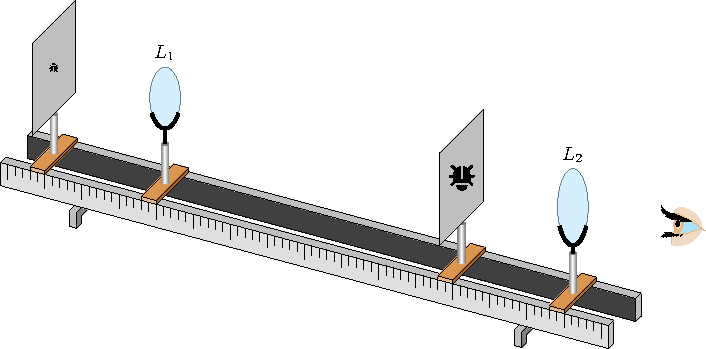
\includegraphics{fig/C/10-8.pdf}
    \caption{}\label{fig_C_10-8}
\end{figure}

用手电筒(或其他光源)照亮玻璃上的小物体,移动物镜
$L_1$,使它到物体的距离$2f_1>u_1>f_1$,同时移动光屏,直到在光
屏上出现小物体清晰的倒立放大的实像.移动目镜$L_2$,同时
通过$L_2$观察光屏上的像,待看到清晰的放大虚像时,移去光
屏,再通过$L_2$观察,这时看到的放大虚像跟有光屏时是一样
的.这表明这个虚像确实是以$L_1$所成的实像为物而产生的.

\section{利用双缝干涉测定光波的波长}

这个实验是利用双缝干涉条纹来测定单色光的波长.实
验装置如图~\ref{fig_C_10-9} 所示.
光源发出的光经滤光片成为单色光.
单色光通过单缝后,经双缝产生干涉.干涉条纹可从屏上观
察到.
\begin{figure}[htbp]
    \centering
    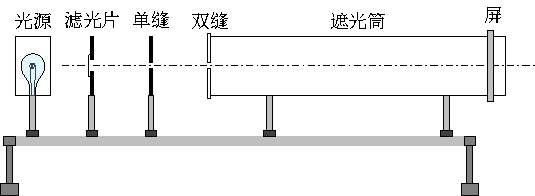
\includegraphics{fig/C/10-9.pdf}
    \caption{}\label{fig_C_10-9}
\end{figure}

双缝间的距离$d$是已知的,双缝到屏的距离$\ell$和相邻两
条干涉条纹间的距离$\Delta x$能够测量,因此可以利用下面的公
式求出波长
\[\lambda=\frac{d\Delta x}{\ell} \]

现在来做实验.把直径约10厘米、长约1米的遮光筒水
平放在光具座上,筒的一端装有双缝,另一端装有毛玻璃屏.
先取下双缝,打开光源,调节它的高度,使它发出的一束光能
够沿着遮光筒的轴线把屏照亮.然后放好单缝和双缝,单缝
和双缝间的距离为$5 \sim 10$厘米,使缝互相平行,中心大致位于
遮光筒的轴线上.这时,在屏上就会看到双缝的干涉条纹.
你看到的干涉条纹是不是彩色的?

放上滤光片,注意观察亮条纹间的距离是否相等.
测出$n$
条干涉条纹间的距离$a$,那么相邻两条干涉条纹间的距离
\[\Delta x=\frac{a}{n-1} \]
再用米尺测出双缝到屏的距离$\ell$.换用另外颜
色的滤光片,观察干涉条纹间的距离有什么变化.

根据已知的双缝间的距离$d$和实验所得的数据,代入公
式求出单色光的波长.

你求出的单色光的波长是多少?利用书中所附的连续光
谱图查出这种波长的光的颜色,跟滤光片的颜色相比较,看着
它们是否一致?

\section{观察光的衍射现象}

\subsection{观察单缝衍射}

用一个具有直长灯丝的白炽灯泡作
线状光源(用距离较远的日光灯管也可以).调节游标卡尺
两脚间的距离,形成一个0.5毫米宽的狭缝.在距灯丝几米远
处,使卡尺的狭缝与直灯丝平行,眼睛紧靠狭缝,通过狭缝观
察线光源.
这时可以看到光通过狭缝后产生的衍射现象:光
束变宽,并有许多条彩色条纹.

调节狭缝的宽度,使它变宽,观察衍射条纹有什么变化;
使狭缝变窄,再观察衍射条纹有什么变化.

\subsection{观察小孔衍射}

用手电筒的小灯泡作点光源.
在铝
箔(或胶片)上打出尺寸不同的小孔.在距点光源$1 \sim 2$米处,
使眼睛紧靠小孔,观察光通过小孔的衍射现象,可以看到彩色
的圆环,孔越小,圆环面积越大.

